\documentclass[12pt]{article}
\usepackage[T1]{fontenc}
\usepackage[latin1]{inputenc}
\usepackage[italian]{babel}
\usepackage{latexsym}
\usepackage{epsfig}
\usepackage{fancybox}
\usepackage{rotating}
\usepackage{graphicx}

\textwidth 15.5cm
\textheight 22.5cm
\topmargin 0cm
\evensidemargin 0in
\oddsidemargin 0in


\def\bbbr{{\rm I\!R}}
\def\bbbm{{\rm I\!M}}
\def\bbbn{{\rm I\!N}}


\def\proof{{{\em Proof:} \/}}
\def\qed{{$\hfill \Box$\\}}

\def\sm{\setminus}
\newcommand {\ol}[1]{\overline{#1}}



\def\La{{\cal \Leftarrow}}
\def\Ra{{\cal \Rightarrow}}


\newtheorem{Teo}{Teorema}[section]
\newtheorem{Con}[Teo]{Congettura}
\newtheorem{Ese}[Teo]{Esercizio}
\newtheorem{Que}{Question}
\newtheorem{Dom}{Domanda}
\newtheorem{Cor}[Teo]{Corollario}
\newtheorem{Property}[Teo]{Propriet\`a}
\newtheorem{Pro}[Teo]{Proposizione}
\newtheorem{Cla}[Teo]{Claim}
\newtheorem{Lem}[Teo]{Lemma}
\newtheorem{Fact}[Teo]{Fatto}
\newtheorem{Def}{Definizione}
\newtheorem{Obs}[Teo]{Osservazione}
\newtheorem{Note}{Nota}
\newtheorem{Prob}{Problema}

% P class
\newcommand{\Pclass}{{\sf\bf P}\xspace}
% NP class
\newcommand{\NPclass}{{\sf\bf NP}\xspace}
% coNP class
\newcommand{\coNPclass}{{\sf\bf coNP}\xspace}
% PSPACE class
\newcommand{\PSPACEclass}{{\sf\bf PSPACE}\xspace}
% MAXSNP class
\newcommand{\MaxSNPclass}{{\sf\bf MaxSNP}\xspace}
% MAXNP class
\newcommand{\MaxNPclass}{{\sf\bf MaxNP}\xspace}
% FPTAS class
\newcommand{\FPTASclass}{{\sf\bf FPTAS}\xspace}
% PTAS class
\newcommand{\PTASclass}{{\sf\bf PTAS}\xspace}
% APX class
\newcommand{\APXclass}{{\sf\bf APX}\xspace}


\pagestyle{empty}
 
\begin{document}
\title{\textbf {Planarit\`a di grafi}}
\author{Note da studente a studente per il corso di Ricerca Operativa prof.~Rizzi\\
Chiara Langella e Romeo Rizzi, 2016}
\date{}
\maketitle
Questa collana di note intende costituire un ulteriore supporto per il corso di Ricerca Operativa del Prof. Rizzi. Gli studenti sono invitati a collaborare al corso con intraprendenza e partecipazione. Proponiamo un possibile canale: la stesura di questa collana di note per coprire zone d'ombra, dove essi abbiano riscontrato delle difficolt\`a.
L'idea \`e che lo studente possa riuscire a parlare ed arrivare in modo pi\`u diretto ai suoi compagni. Il docente pu\`o riorganizzare spiegazioni e materiali sulla proposta dello studente e guidarlo nella stesura di un documento utile, corretto, ed efficace.

\section{Un puzzle come apetizer}

Con 3 case e 3 risorse (acqua, luce e gas)
viene spesso proposto un celebre problema matematico che scommetto avrete incontrato anche voi da ragazzi:

\begin{quote}
Si supponga di avere tre villini collocati nel piano.
Ciascuno di essi vuole allacciarsi sia alla compagnia dell'acqua, che a quella della luce, che a quella del gas.
Senza utilizzare la terza dimensione, n\`e far passare una delle connessioni attraverso un'altro villino o compagnia, vi risulta possibile realizzare tutte e 9 le connessioni senza che le linee finiscano per incrociarsi?
\end{quote}


% VERSIONE INGLESE (meglio tenerle quando le abbiamo, non e` detto che non si vorra` curare anche delle traduzioni in inglese per gli studenti stranieri)
%
%The classical mathematical puzzle known as the three utilities problem; the three cottages problem or sometimes water, gas and electricity can be stated as follows:

%\begin{quote}
%Suppose there are three cottages on a plane (or sphere) and each needs to be connected to the gas, water, and electricity companies. Without using a third dimension or sending any of the connections through another company or cottage, is there a way to make all nine connections without any of the lines crossing each other?
%\end{quote}

\begin{figure}[!ht]
\centering
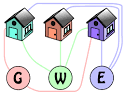
\includegraphics[width=0.30\textwidth]{3houses.png}
 \quad 
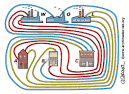
\includegraphics[width=0.30\textwidth]{3factories.png}                   
 \quad 
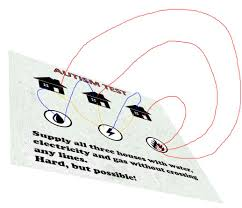
\includegraphics[width=0.30\textwidth]{3Dsolution.jpg}
\caption{A sinistra: il puzzle. In centro: una soluzione farlocca. A destra: soluzione se si potesse uscire dal piano.}
\end{figure}



Lasciatevi affascinare dal materiale e dalle soluzioni bizzarre alla pagina:
\begin{verbatim}
    http://www.archimedes-lab.org/How_to_Solve/Water_gas.html
\end{verbatim}
Sulla storia del puzzle speravo di trovare di pi\`u alla pagina di Wikipedia:
\begin{verbatim}
     https://en.wikipedia.org/wiki/Three_utilities_problem
\end{verbatim}


\section{Teoria}

Il puzzle offre un problema che presenta una doppia natura:
topologica e combinatoria.
L'aspetto topologico \`e evidente: stiamo chiedendo se sia possibile tracciare un certo disegno nel piano.
La natura combinatoria diventa pi\`u esplicita osservando come
il problema possa trovare efficace rappresentazione nel linguaggio della teoria dei grafi.
Gli oggetti del contendere (3 case e 3 compagnie) possono essere visti
come 6 nodi (3 di un tipo e 3 di un altro), mentre le 9 richieste di garantire una connessione diretta tra ogni casa ed ogni compagnia trovano rappresentazione in 9 archi. Ciascuno di questi 9 archi ha un estremo in una casa e l'altro in una compagnia, e pertanto siamo al cospetto di un grafo bipartito.
Pi\`u precisamente ad un grafo bipartito e completo, dato che ogni casa chiede di essere connessa ad ogni compagnia.

Componendo questo grafo, il puzzle ci appare ora un'istanza particolare di un problema pi\`u generale:
dislocare nel piano un certo numero di entit\`a e progettarne la struttura in modo da garantire il contatto diretto tra due entit\`a ove richiesto. Ad esempio, anni or sono all'architetto Mario fu chiesto di realizzare 5 stanze nel bunker del Pentagono, e si voleva che ogni due stanze fossero collegate da una porta.
Il problema di Mario trova rappresentazione in un grafo di 5 nodi. Il grafo di Mario \`e completo: presenta un arco per ogni possibile coppia di nodi in quanto ogni due delle stanze devono essere adiacenti, ossia avere una parte di parete in comune dove risieda la porta privata tra di loro.

In entrambi i casi, l'istanza del problema \`e diventata un grafo ($K_{3,3}$ o $K_5$) ossia un oggetto finito della matematica discreta. E questo oggetto finito tiene stretto in pugno il nocciolo del problema topologico.

La nostra attenzione si volge al seguente problema algoritmico:

\begin{Prob}[{\sc Planarity}]
   Dato un grafo, decidere se esso ammetta un planar drawing dove gli archi non si incrocino.
\end{Prob}  

La seguente figura propone una sequenza di possibili drawings del $K_{3,3}$ nel piano, partendo a sinistra con un drawing suggerito dalla formulazione del puzzle stesso, e cercando di ridurre via via il numero di incroci tra le linee. 

\begin{figure}[!ht]
\centering
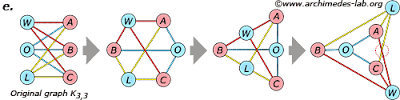
\includegraphics[width=0.90\textwidth]{K33drawings.png}
 \quad 
\caption{Alcuni possibili drawings del $K_{3,3}$.}
\end{figure}


Un grafo � \emph{planare} se lo si pu� disegnare nel piano senza che nessuno dei suoi archi si incroci.
Se un grafo � planare � possibile fornirne un \emph{planar embedding},
cio\`e un disegno (drawing) nel piano dove due archi possono condividere solo i loro punti estremi (ossia i nodi cui fanno capo).

Non tutti i grafi sono planari. Due celebri esempi sono il $K_5$ ed il $K_{3,3}$.
In internet o nei libri potete trovare diverse dimostrazioni del fatto che $K_5$ e $K_{3,3}$ non sono planari, e noi collezioneremo alcune di queste dimostrazioni in appendice al presente documento. Nel seguito daremo per conoscenza ormai assodata e condivisa la non-planarit\`a di $K_5$ e $K_{3,3}$.

\begin{figure}[!ht]
\centering
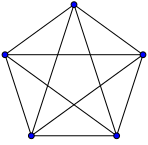
\includegraphics[width=0.30\textwidth]{K5.png}
 \quad 
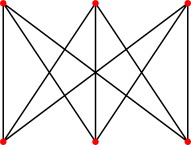
\includegraphics[width=0.30\textwidth]{K3,3.png}
\caption{$K_5$ a sinistra, $K_{3,3}$ a destra.}
\end{figure}
                  
                      
In generale, il $K_n$ � l'unico grafo con $n$ nodi e tutti gli ${n \choose 2}$ archi; esso � planare per $n\leq 4$.
Invece il $K_{m,n}$ � l'unico grafo bipartito (=bicolorabile), con $m$ nodi rossi ed $n$ nodi blue, e tutti i possibile $m\times n$ archi con estremi di colore diverso; esso � planare per $\min\{m,n\} \leq 2$.

Ovviamente, un modo semplice ed efficace per convincere/convincersi
che un grafo \`e planare consiste appunto nel fornirne un planar embedding.

\begin{Ese} \label{ese:planarSI1}
    Si dimostri che $K_n$ � planare per ogni $n \leq 4$.
\end{Ese}

\begin{Ese}
    Si dimostri che $K_{m,n}$ � planare se $\min\{m,n\} \leq 2$.
\end{Ese}

Il fatto che sia facile fornire evidenza (ossia verificabile riscontro) della planarit\`a di un grafo significa il problema algoritmico
{\sc Planarity} \`e in {\sf\bf NP}; il certificato \`e il planar embedding.
La degna sfida per il matematico \`e pertanto quella di porre il problema in {\sf\bf coNP}, ossia venire a conoscere il linguaggio del NO.

\begin{Que}
Quale tipo di argomentazione risulter\`a sempre efficace al convincere che un grafo assegnatoci non \`e planare?
\end{Que}

La risposta a questa domanda venne col teorema di Kuratowski (1930) che per varie ragioni \`e destinato a rimanere una pietra miliare nella storia della matematica, e tuttavia non rinunceremo a fare i nostri passetti di esplorazione per meglio impadronirci dei concetti che si sono rivelati pi\`u significativi.


Nell'Esercizio~\ref{ese:planarSI1},
\`e parlare come si mangia fornire un planar embedding
per il solo caso di $n=4$, perch\`e mi sa tanto che se $K_4$ \`e planare allora anche $K_3$, e $K_2$, e anche $K_1$ dovranno pur esserlo, no?
Una possibile ragione che sottintende queste utili implicazioni  \`e che $K_{p}$ \`e un sottografo di $K_{q}$ se $p\leq q$,
e quindi ci\`o che viene in nostro soccorso sono la definizione ed il lemma seguente.

\begin{Def} \label{def:sottografo}
    Siano $G=(V,E)$ e $H=(V',E')$ due grafi con $V'\subseteq V$ e $E'\subseteq E$. Diremo allora che $H$ \`e un sottografo di $G$.
\end{Def}

\begin{Lem} \label{ese:planarSI1}
    Sia $H$ un sottografo di $G$. Se $H$ non \`e planare allora nemmeno $G$ lo \`e.
\end{Lem}
\proof
   Dimostrazioni come queste poggiano tipicamente sui certificati.
   Si assuma, per assurdo, che $G$ sia planare, e si consideri quindi un suo certificato di planarit\`a, ossia un planar embedding di $G$.
   L'intuizione \`e che tale planar embedding conterr\`a dentro di s\`e un planar embedding di $H$ (ossia un certificato di planarit\`a per $H$, ottenendo la contraddizione con l'assunzione che $H$ non \`e planare).
   Il livello di formalismo pi\`u opportuno dipender\`a dal contesto. 
\qed

La propriet\`a di planarit\`a gode quindi della seguente monotonia.

\begin{Fact} \label{fact:monotony}
 La planarit\`a non pu\`o essere distrutta per rimozione di archi.
\end{Fact}

Fact~\ref{fact:monotony}
motiva lo studio di come possano essere fatti i grafi non-planari minimali, ossia grafi non planari dove per\`o la rimozione di un qualsiasi arco conduca ad un grafo planare.

\begin{Ese}
    Si dimostri che $K_5$ � non-planare minimale.
\end{Ese}

\begin{Ese}
    Si dimostri che $K_{3,3}$ � non-planare minimale.
\end{Ese}

\begin{Que}
    Esistono altri grafi non-planari minimali oltre a $K_5$ e $K_{3,3}$?
    Il loro numero \`e finito?
\end{Que}

Nel considerare l'operazione di rimozione di archi non potr\`a sfuggire che se ad un certo punto non vi \`e alcun arco incidente in un certo nodo, allora tale nodo \`e del tutto inessenziale al problema {\sc Planarity} e pu\`o quindi essere rimosso in bella partenza.
I nodi di grado zero non possono contribuire nel determinare se un grafo sia planare o meno.

\begin{Que}
    E i nodi di grado uno?
    Possiamo rimuovere anche loro senza che la propriet\`a di planarit\`a ne risulti affetta?
\end{Que}

In effetti s\`\i, se rimuoviamo un nodo e l'unico arco in esso incidente otteniamo un nuovo grafo che \`e planare se e solo se lo era il grafo di partenza.

\begin{Que}
    E i nodi di grado due?
    Possiamo rimuovere anche loro senza che la propriet\`a di planarit\`a ne risulti affetta?
    Che operazione suggeriresti di effettuare per sbarazzarti di un nodo di grado due ottenendo un nuovo grafo che \`e planare se e solo se lo era il grafo di partenza?
\end{Que}

\begin{Def}
   Due archi si dicono \emph{in serie} se hanno in comune un nodo di grado due nel grafo di riferimento.
   Dati due archi in serie $ab$ e $bc$, si chiama \emph{splitting off}
   l'operazione che consiste nel rimuovere il nodo $b$ e rimpiazzare
   i due archi $ab$ e $bc$ col solo arco $ac$.       
   L'operazione inversa \`e la \emph{suddivisione di un arco} e consiste nell'inserire un nuovo nodo nel mezzo dell'arco (che viene poi visto come due archi in serie).
   Un grafo $G$ \`e \emph{una suddivisione} di un grafo $H$ se e solo se pu\`o
essere ottenuto da $H$ tramite una sequenza di suddivisioni.
\end{Def}

\begin{Obs}
   Se $G$ \`e una suddivisione di $H$ allora $G$ \`e planare se e solo se $H$ \`e planare. Inoltre, $G$\`e non-planare minimale se e solo se $H$ lo \`e.
\end{Obs}

\begin{Que} \label{que:criticalChar}
    Le infinite suddivisioni di $K_5$ e $K_{3,3}$
    sono i soli grafi non-planari minimali?
\end{Que}

Le infinite suddivisioni di $K_5$ e $K_{3,3}$ vengono chiamate \emph{grafi di Kuratowski}. 
Non mi \`e noto se la Question~\ref{que:criticalChar} sia mai stata posta in questi termini, e tuttavia una buona caratterizzazione della proprit\`a di planarit\`a
fu comunque ottenuta col seguente:

\begin{Teo} \label{teo:Kuratowski}
    Un grafo \`e planare se e solo se non contiene alcun grafo di Kuratowski
    come sottografo.
\end{Teo}

\begin{Ese} \label{ese:planarSI1}
    Si dimostri che la risposta alla Question~\ref{que:criticalChar}
    \`e positiva avvalendosi del teorema di Kuratowski.
\end{Ese}

Di fatto, il teorema di Kuratowski ricompose importanti e solidi legami tra la topologia e la teoria dei grafi:
due discipline che, scaturite dal lavoro di Eulero (1736) sul problema dei sette ponti di K\"onigsberg, avevano preso poi ciascuna la sua strada.

Del 1931 \`e una riformulazione equivalente del teorema di Kuratowski dovuta a Wagner.

\begin{Teo} \label{teo:Wagner}
    Un grafo \`e planare se e solo se non contiene un $K_5$ od un $K_{3,3}$ minor.
\end{Teo}

Anche se non \`e difficile mostrare l`equivalenza dei Teoremi~\ref{teo:Wagner} e~\ref{teo:Kuratowski}, enorme fu l'influenza del lavoro di Wagner negli sviluppi e nelle rivoluzioni che ne seguirono nella graph theory e pi\`u in ampio.

\section{Pratica} 

La richiesta base � quella di certificare se il grafo dato sia planare o meno.

Pertanto una volta che avrete \emph{intuito} se il grafo dato � planare o no, bisogna fornirne il relativo certificato e vi si possono presentare due casi:

\begin{itemize}
\item Se il grafo � \textbf{planare} allora il relativo certificato consiste solo nel disegnare il grafo \emph{planarizzato}(ovvero disegnarlo senza incrociare gli archi).\\
\item Se il grafo \textbf{non � planare} bisogna individuare o un $K_{3,3}$ o un $K_5$ \footnote{mostrati in figura 3} al suo interno. Questo pu� risultare pi� complicato. Si consideri il caso in cui si voglia individuare un $K_{3,3}$: � necessario selezionare tre nodi 'maschi' (colorateli di blu) e tre nodi 'femmine' (colorateli di rosso) e mostrare che da ogni nodo blu si raggiungono tutti e tre i nodi rossi. \emph{Non} � strettamente necessario che vi sia un solo arco che collega il primo nodo maschio a ciascuna femmina, ma � importante che tutti e sei i differenti percorsi non condividano nessun nodo e quindi nessun arco in comune. 
\end{itemize}

\subsection{Esempio: problema 6, esame del 28/09/2016}
Si chiedeva di stabilire se fosse planare o meno il grafo $G$ in figura qu\`\i\ sotto,
ma anche il grafo $G'$ ottenuto da $G$ sostituendo l'arco $hx$ con $qx$. 
\begin{figure}[htb]   % h=here; t=top; b=bottom;
\begin{center}
  \leavevmode
  \psfig{figure=input.pdf, height=7.0 true cm}
\end{center}
\end{figure}

Come per la maggior parte degli altri esercizi, non \`e questione di rispondere con dei SI o dei NO, ma di fornire i certificati che suffraghino le vostre conclusioni.
Trovate un certificato di planarit\`a di $G$ (un planar embedding di $G$) nella correzione ufficiale, pi\`u delicato \`e come si possa certificare il NO.
Occorre fare riferimento al teorema di Kuratowski e scopo del presente documento \`e chiarire per bene come, quali siano le modalit\`a corrette a prevenire errori tipici e ricorrenti.
Rimandiamo nuovamente alla correzione ufficiale per un certificato di non planarit\`a di $G'$ come sconfifferi al prof (nostro Re Art\`u). 

Quello che vogliamo sottolineare qu\`\i\ \`e come vadano messi in cassaforte i punti della non-planarit� all'esame.
Per prima cosa quello che dovete ricordarvi � che \textbf{se non fornite il certificato non ottenete i punti!} Questi infatti vengono assegnati solo se fornite il certificato. Tale certificato deve, tuttavia, essere corretto: ovvero offrire effettivamente il risontro di una suddivisione di $K_{3,3}$ o di $K_5$ entro $G'$, non basta dire ``$G'$ non \`e planare perch\`e contiene una suddivisione di $K_{3,3}$'', chi crediamo di prendere in giro? Dobbiamo mettere in bella evidenza una tale suddivisione di $K_{3,3}$ o di $K_5$ entro $G'$. Per altro queste suddivisioni non sono uniche.
Gli esempi di errori pi� comuni sulla non-planarit� sono i seguenti:
\begin{itemize}
\item \textbf{Incrocio di archi}: evidenziare che due archi si incrociano in un particolare disegno del grafo $G'$ non equivale ad un certificato di non-planarit�. Non basta un disegno fallace, si chiede di mostrare che comunque ci si ingegni il disegno sar\`a condannato ad essere fallace. 
\item \textbf{Mancanza del certificato}: se si disegna il grafo $G'$ e si afferma solo che il grafo non � planare senza alcuna giustificazione, oppure senza un riscontro che consenta a Re Art\`u la verifica. Se dite che $G'$ contiene un $K_5$ mostrate dove siano i $5$ nodi importanti di questo $K_5$, e non solo ...\\ 
\item \textbf{Cammini tra i 6 nodi del $K_{3,3}$ non specificati}: questo � il caso in cui si evidenzino i $6$ nodi importanti del $K_{3,3}$, magari specificandone anche il lato della bipartizione (come richiesto!), ma senza tracciare i cammini che conducono i $3$ 'nodi maschi' dai $3$ 'nodi femmina'.
Esperienza a correggere numerosi compiti insegna che il pi\`u delle volte che si lascino questi cammini fantasma \`e perch\`e lo studente ha scelto male i $6$ nodi, se non addirittura aveva sbagliato nell'optare per il $K_{3,3}$ invece che per il $K_{3,3}$ (frequente anche il viceversa).\\

\item \textbf{Cammini con nodi interni in comune}: � il caso della seguente figura in cui i nodi triangolati in viola sono in comune:
\begin{center}
  \psfig{figure=wrongplanarity.pdf, height=7.0 true cm}
\end{center}
ad esempio il nodo \emph{t} � nodo in comune, in quanto appartiene sia al percorso che porta dal nodo $p$ al nodo $d$, sia al percorso da $p$ a $q$.\\
Se consentissimo alle suddivisioni di $K_5$ o $K_{3,3}$ di condividere nodi interni ai cammini allora esse non funzionerebbero pi\`u come strumento atto a certificare la non-planarit\`a e in realt\`a non starei certificando proprio nulla.
Ad esempio, chi oserebbe dire che la seguente ``suddivisione di $K_5$ con nodo interno $x$ messo in comune a due cammini non \`e un grafo planare?

\begin{center}
  \psfig{figure=planarK5subdivision.pdf, height=6.0 true cm}
\end{center} 
Si rilegga la definizione di suddivisione data sopra e si realizzi una volta per tutte che la suddivisione di $K_5$ in figura tanto suddivisione non \`e.

\item \textbf{Cammini con un nodo interno che si colloca su un nodo importante}:
anche questo \`e da furbetti e non funzia a dovere come certificato, come evidenziato nella seguente soluzione creativa al rendere planare un circuito che non vuole esserlo:

\begin{figure}[!ht]
\centering
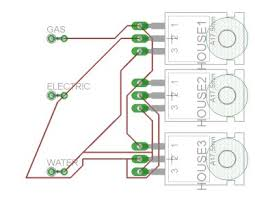
\includegraphics[width=0.60\textwidth]{goThroughNodeCircuitSolution.jpg}
 \quad 
\caption{Una soluzione che bara: ai cammini privati non \`e concesso n\`e di incontrarsi se non nei nodi ``importanti'' che collegano (internally node disjoint) ne`di passare per altri nodi ``importanti'' per scavalcare altri cammini.}
\end{figure}

Si rilegga la definizione di planarit\`a dando un peso alle parole:
\begin{quote}
Se un grafo � planare � possibile fornirne un \emph{planar embedding},
cio\`e un disegno (drawing) nel piano dove {\bf due archi possono condividere solo i loro punti estremi (ossia i nodi cui fanno capo)}.
\end{quote}

\end{itemize} 


Sappiate che in tutti i casi sopra elencati NON si ottengono punti! 


\section{Altre risorse e materiali che suggeriamo di visionare}

Trovate in www un bel video sul teorema di Kuratowski:\\
\begin{verbatim}
   https://www.youtube.com/watch?v=UkjJE3bmPV0
\end{verbatim}
Di fatto questo video fa parte di una collana (canale)
di video in graph theory\\
\begin{verbatim}
   https://www.youtube.com/watch?v=eIb1cz06UwI&list=PLoJC20gNfC2gmT_5WgwYwGMvgCjYVsIQg
\end{verbatim}




\end{document}
